\section{Analytical results}

The system studied for this report is a simple pendulum of mass \(m=0.2\) kg attached to a rod of time-dependent length
\begin{equation}
    \ell(t) = L + \alpha t + d \sin (\omega t)
\end{equation}
where \(L=0.2\) m and the other parameters are set depending on the simulation. The mass experiences a downwards acceleration due to gravity \(\vec{g}=-g \vec{e_y}\) and a tension force due to the rod \(\vec{T} = T \vec{e_r}\), where \(\vec{e_x}\), \(\vec{e_y}\) are the basis vectors of a carthesian coordinate system centered in \(\mathcal O\) and \(\vec{e_r}\), \(\vec{e_\theta}\) the basis vectors of a polar coordinate system, as shown in \autoref{fig:system_schematic}.

\begin{figure}[h]
    \centering
    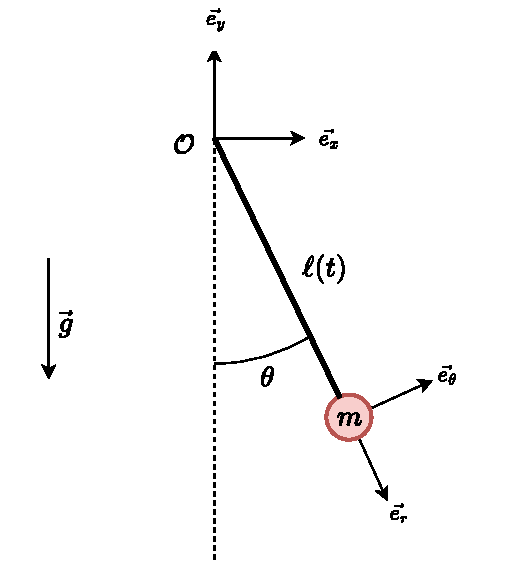
\includegraphics[width=0.6\linewidth]{figures/system_schematic.pdf}
    \caption{A simple pendulum of mass \(m\) and variable length \(\ell(t)\)}
    \label{fig:system_schematic}
\end{figure}

\subsection{System of differential equations}
\underline{Question (a)}

Let us take the vector: $\textbf{y} = (\theta, \dot\theta)$

We are searching for $f$ such that:
\begin{equation}
    \frac{\dd \textbf{y}}{\dd t} = \left(\begin{matrix} \dot\theta \\ \ddot\theta \end{matrix}\right) = f(\textbf{y})
    \label{eq:a_question}
\end{equation}

The forces applied on the mass expressed in the polar coordinate system \(\vec{e_r}, \vec{e_\theta}\) are
\begin{equation}
    \vec{g} = g \cos(\theta) \vec{e_r} - g \sin(\theta) \vec{e_\theta}
\end{equation}
\begin{equation}
    \vec{T} = T \vec{e_r}
\end{equation}
where \(g=9.81\) \si{\meter\per\second} and \(T\) is the (signed) norm of the tension force. Using the formulae for acceleration in polar coordinates we obtain the following equations of motion
\begin{equation}
    \begin{cases}
        m(\ddot\ell(t) - \ell(t) \dot\theta^2) = mg\cos(\theta) + T \\
        m(\ell(t)\ddot\theta + 2\dot\ell(t) \dot\theta) = -mg\sin(\theta)
    \end{cases}
    \label{eq:motion}
\end{equation}
By rearanging these equations, we obtain
\begin{equation}
    \begin{cases}
        \dot\theta = \pm \sqrt{\frac{-g\cos(\theta) - \frac{T}{m} + \ddot\ell(t)}{\ell(t)}} \\
        \ddot\theta = \frac{-g\sin(\theta) - 2\dot\ell(t) \dot\theta}{\ell(t)}
    \end{cases}
    \label{eq:thetadot_thetadotdot}
\end{equation}
which allows us to rewrite \autoref{eq:a_question} as
\begin{equation}
    \frac{\dd \textbf{y}}{\dd t} = f(\textbf{y}) = \left(\begin{matrix}
        \pm \sqrt{\frac{-g\cos(\theta) - \frac{T}{m} + \ddot\ell(t)}{\ell(t)}} \\
        \frac{-g\sin(\theta) - 2\dot\ell(t) \dot\theta}{\ell(t)}
    \end{matrix}\right)
    \label{eq:ode}
\end{equation}

\subsection{Mechanical energy}
\underline{Question (b)}

We are searching for the total mechanical energy of the system. By considering the mass as a point mass, we can write the total mechanical energy as the sum of the translational kinetic energy and the potential
\begin{equation}
    \begin{aligned}
        \mathrm{E_{tot}} &= \frac{1}{2}mv^2 - mgy \\
        &= \frac{1}{2}m(\ell(t)^2 \dot\theta^2 + \dot\ell(t)^2) - mg\cos(\theta)
    \end{aligned}
\end{equation}
This energy is not conserved. The gravitational potential is conserved as gravity is a central force. However, the tension does not derive from a potential and does produce work, as the mass does move along the \(\vec{e_r}\) direction, which means it is not conserved. The power of this non-conservative force is given by
\begin{equation}
    \begin{aligned}
        P &= \vec{T} \cdot \vec{v} \\
        &= T \dot\ell(t)
    \end{aligned}
\end{equation}
Using the first equation from \autoref{eq:thetadot_thetadotdot}, we can express \(T\) as
\begin{equation}
    T = m(\ddot\ell(t) - g\cos(\theta) - \dot\theta^2 \ell(t))
\end{equation}
which gives us the final expression for the power
\begin{equation}
    P = m(\ddot\ell(t) - g\cos(\theta) - \dot\theta^2 \ell(t)) \dot\ell(t)
\end{equation}

\subsection{Specific solution for constant length rod}
\label{sec:analytic:constant_length}
\underline{Question (c)}

For this part we will set \(\alpha=0\) and \(d=0\), meaning the length of the pendulum remains constant (\(\ell(t)=L\)). We assume small movements around the stable equilibrium position, i.e. \(\theta \ll 1\). Under this assumption, we can write \(\sin(\theta) \approx \theta\) and \(\cos(\theta) \approx 1\). The equations of motion from \autoref{eq:motion} then become
\begin{equation}
    \begin{cases}
        -m L \dot\theta^2 = mg\cos(\theta) + T = mg + T \\
        m L \ddot\theta = -mg\sin(\theta) = -mg\theta
    \end{cases}
\end{equation}
from which we get
\begin{equation}
    \ddot\theta = - \underbrace{\frac{g}{L}}_{\omega_0^2} \theta
\end{equation}
which is the equation for a harmonic oscillator. The general solution is given by
\begin{equation}
    \theta(t) = A\cos(\omega_0 t) + B\sin(\omega_0 t)
\end{equation}
Imposing the intial conditions \(\theta(0) = \theta_0\) and \(\dot\theta(0) = 0\), we find \(A = \theta_0\) and \(B = 0\). The solution for this case is thus given by
\begin{equation}
    \theta(t) = \theta_0 \cos(\omega_0 t)
\end{equation}
